\documentclass{article}
\usepackage{fullpage}
\usepackage{amsmath}
\usepackage{amsfonts}
\usepackage{authblk,caption}
\usepackage{titling}
\usepackage{tikz}
\usepackage{hyperref}
\usepackage{graphicx}
\graphicspath{{images/}}
\title{\huge{Classical Mechanics 1, Autumn 2021 CMI \\ Problem set 7\\\hspace{7cm}- Govind S. Krishnaswami}
}
\author{Soham Chatterjee\\Roll: BMC202175}
\date{}
\newcommand{\mcR}{\mathcal{R}}
\newcommand{\bma}{\boldsymbol{a}}
\newcommand{\bmb}{\boldsymbol{b}}
\newcommand{\bmc}{\boldsymbol{c}}
\newcommand{\bmr}{\boldsymbol{r}}
\newcommand{\bmv}{\boldsymbol{v}}
\newcommand{\bmp}{\boldsymbol{p}}
\newcommand{\bmF}{\boldsymbol{F}}
\newcommand{\bmB}{\boldsymbol{B}}
\newcommand{\bmf}{\boldsymbol{f}}
\renewcommand\maketitlehooka{\null\mbox{}\vfill}
\renewcommand\maketitlehookd{\vfill\null}

\setlength{\parindent}{1cm}
\begin{document}
	\maketitle\pagebreak
	\begin{enumerate}
		\item \begin{enumerate}
			\item Given that $x(t)=\Re \left[Ae^{i\omega t}\right]$ where $A$ is a complex number. Let $A=m+in$. Hence \begin{align*}
				x(t)\ &=\Re\left[(m+in)e^{i\omega t}\right]\\
				&= \Re\left[m\cos (\omega t) - n\sin(\omega t)+i(m\sin(\omega t)+n\cos(\omega t))\right]\\
				&= m\cos (\omega t) - n\sin(\omega t)\\
				&=\sqrt{m^2+n^2}\left( \frac{m}{\sqrt{m^2+n^2}} \cos(\omega t)-\frac{n}{\sqrt{m^2+n^2}}\sin(\omega t)\right)\\
				&=\sqrt{m^2+n^2}\cos(\omega t +\alpha)\\
				&=|A|\cos(\omega t +\alpha)
			\end{align*}where $\cos\alpha=\frac{m}{\sqrt{m^2+n^2}}$ and $\sin\alpha=\frac{n}{\sqrt{m^2+n^2}}$. 	
		Hence amplitude of the simple harmonic motion is $|A|$.
		
		\item $\cos\alpha=\frac{m}{\sqrt{m^2+n^2}}$ and $\sin\alpha=\frac{n}{\sqrt{m^2+n^2}}$. 	Hence\begin{align*}
			& \tan\alpha\ = \frac{n}{m}\\
			\implies & \alpha=\tan^{-1}\frac{n}{m}=\arg A
		\end{align*}Hence the initial phase $\alpha$ of the motion is $\arg A$.
	\item $x(t)=|A|\cos(\omega t +\alpha)=m\cos (\omega t) - n\sin(\omega t)$. Hence $\dot{x}(t)=-|A|\omega\sin(\omega t +\alpha)=-m\omega\sin(\omega t)-n\omega\cos(\omega t)$. Therefore \begin{align*}
		x(0)\ &=m\cos(\omega\times 0)-n\sin(\omega \times 0)=m\cos 0 -n\sin 0=m=\Re(A)\\
		& =|A|\cos(\omega \times 0 +\alpha)=|A|\cos\alpha\\
		\dot{x}(0)\ &=-m\omega\sin(\omega\times 0)-n\omega\cos(\omega \times 0)=-m\omega\sin 0 -n\omega\cos 0=-n\omega=-\omega\Im(A)\\
		&= -|A|\omega\sin(\omega \times 0 +\alpha)=-|A|\omega\sin\alpha
	\end{align*}
		\end{enumerate}
	\item \begin{enumerate}
		\item Given that $V(x)=\lambda(x^2-a^2)^2=\lambda(x-a)^2(x+a)^2$\begin{figure}[h]
			\centering
			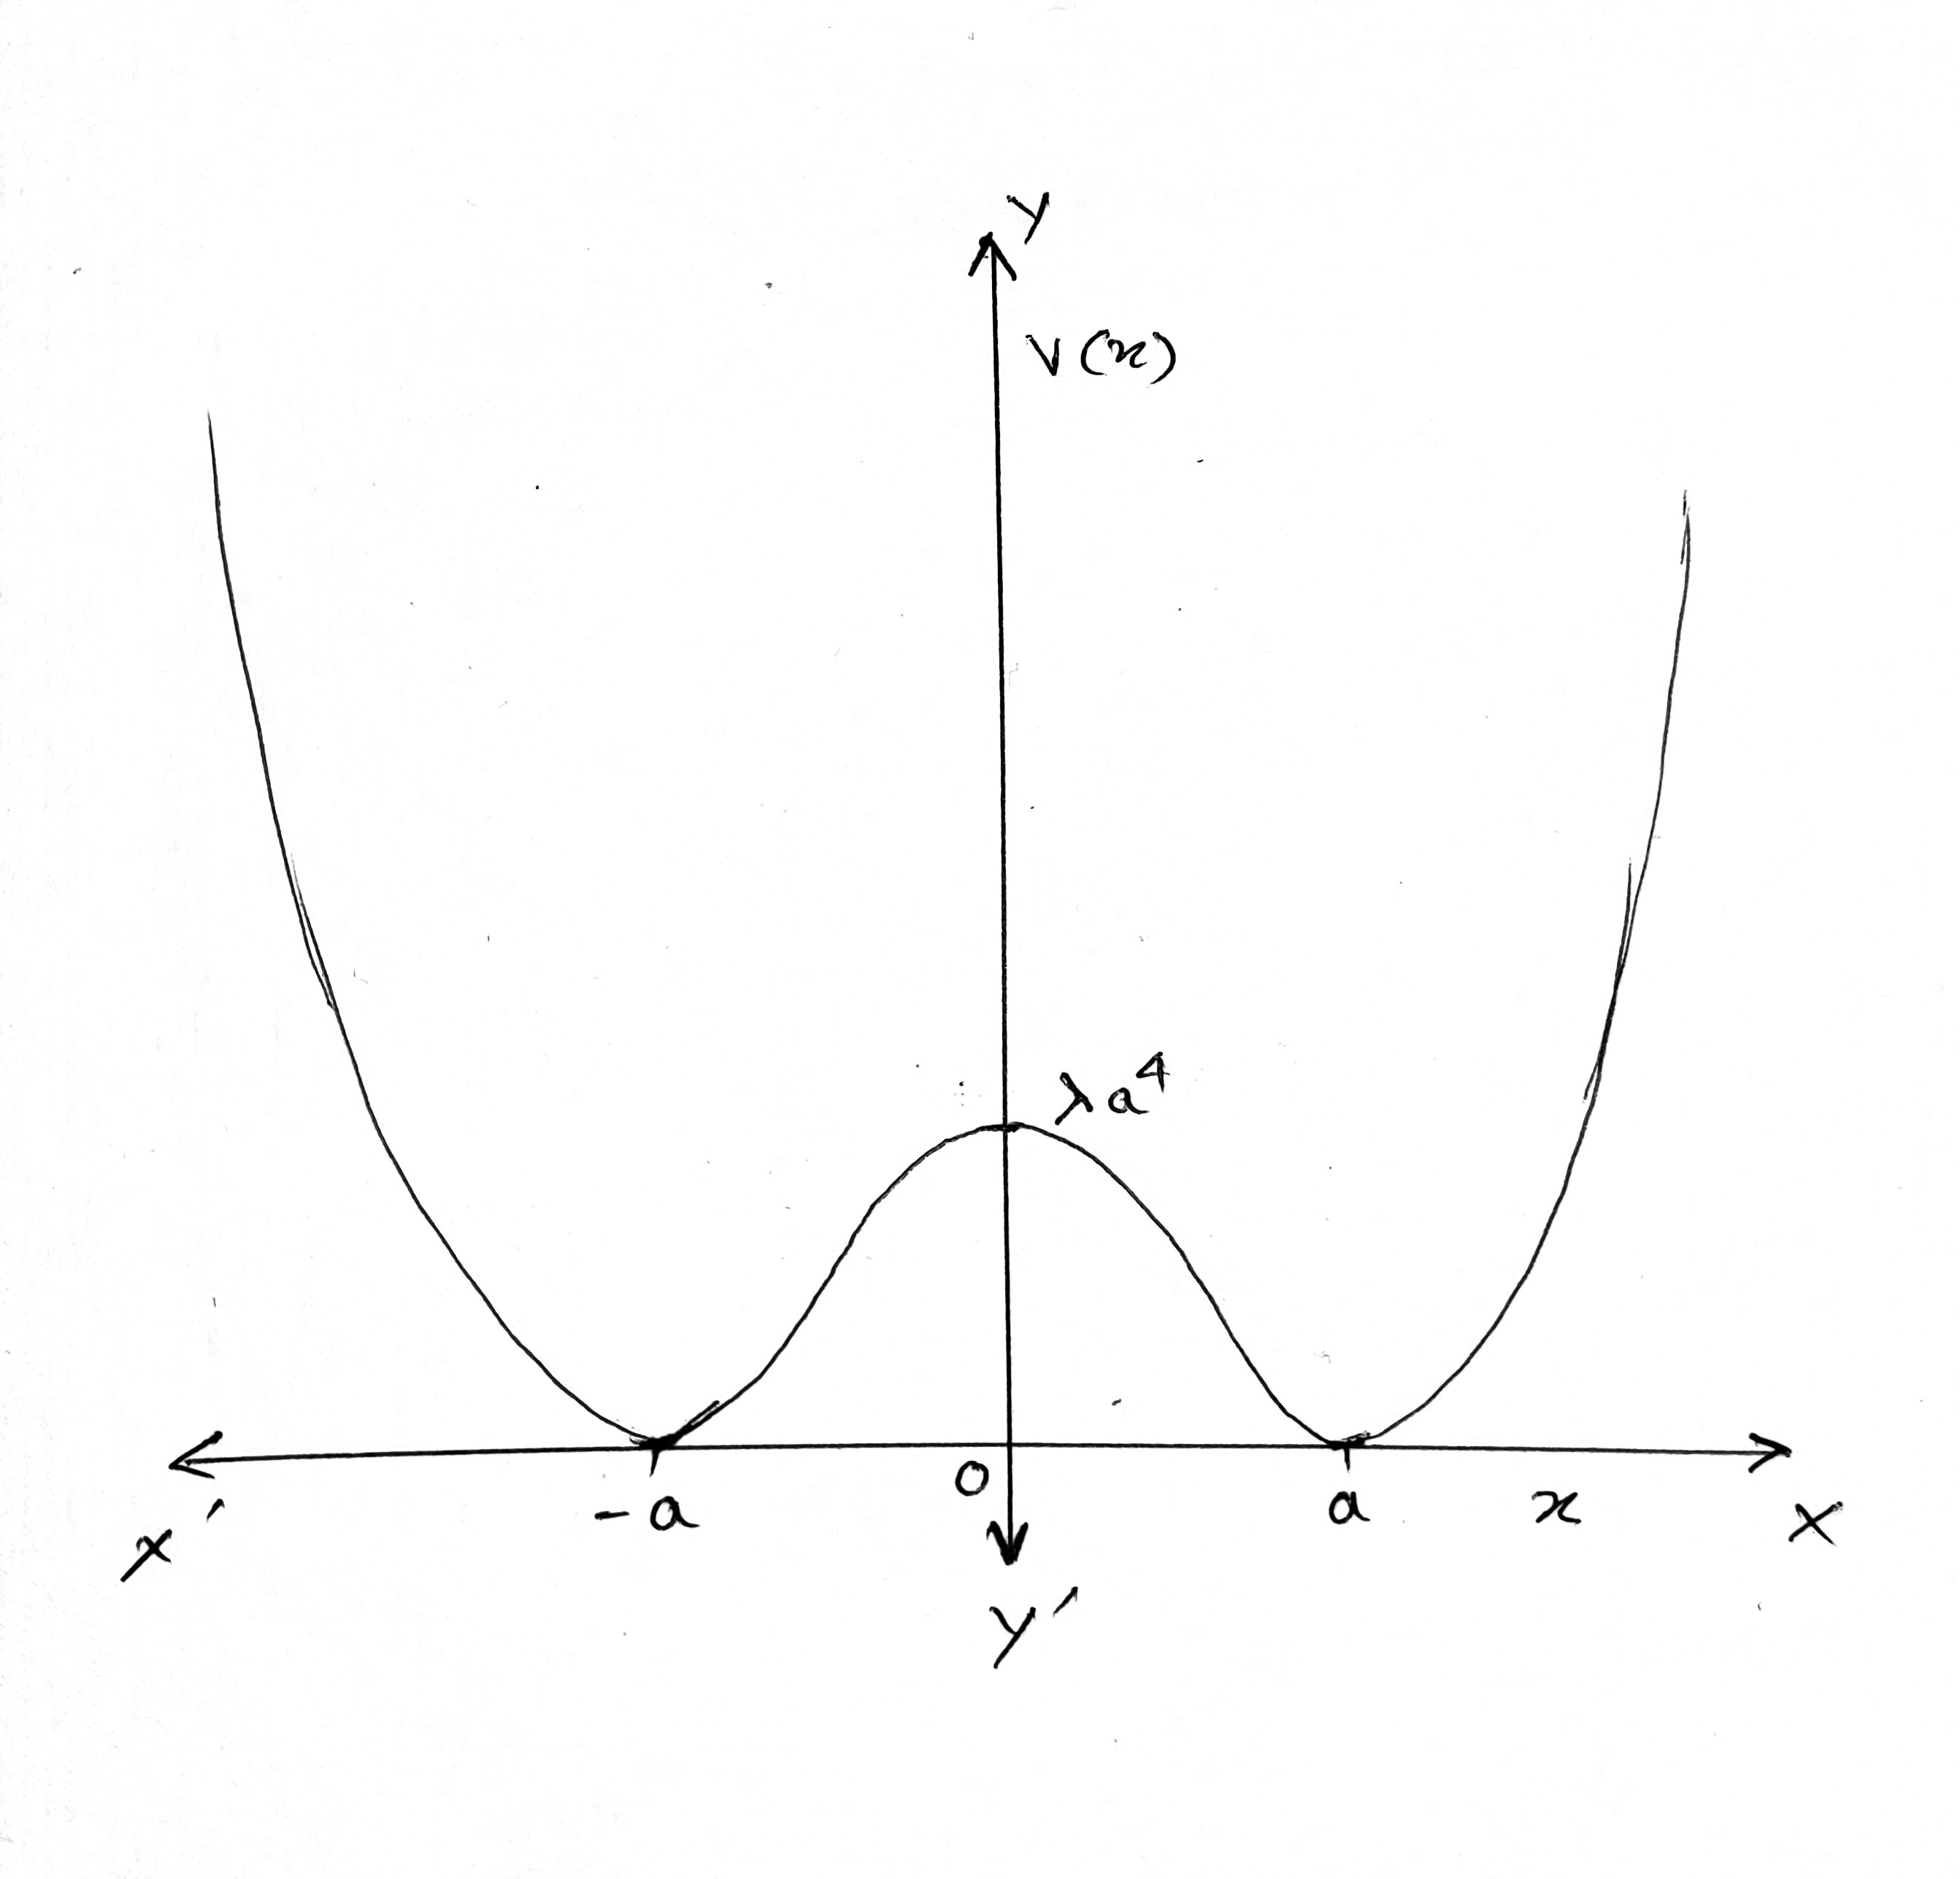
\includegraphics[width=8cm]{1.jpg}
			
		\end{figure}
	\item For static solution $\frac{d}{dx}V(x)=0$. Therefore \begin{align*}
		& \frac{d}{dx}\lambda(x^2-a^2)^2=0\\
		\implies & 4\lambda(x^2-a^2)x=0\\
		\implies & 4\lambda x(x-a)(x+a)=0
	\end{align*}Hence the static solutions are $x=0,a,-a$. 
\item At $x=a,-a$ $V(x)=0$. And at $x=0$ $V(x)=\lambda a^4\neq 0$. Hence $a,-a$ are stable solutions and $0$ is unstable solution.
	\end{enumerate}
	
	
	
	\item $x_1,x_2$ are neighboring turning points. Hence the time interval between the two positions is $\frac{T}{2}$ where $T$ is the time period of the oscillation. Hence when $x=x_1, x_2$, $E(x)=V(x)$ and when $x_1<x<x_2$, $V(x)<E(x)$. Hence $E(x)=V(x)+\frac12m\dot{x}^2$. \begin{align*}
	& E(x)=V(x)+\frac12m\dot{x}^2\\
	\implies & \frac12m\dot{x}^2=E(x)-V(x)\\
	\implies & \frac{dx}{dt}=\sqrt{\frac{2(E(x)-V(x))}{m}}\\
	\implies & \sqrt{\frac{m}{2}}\frac{dx}{\sqrt{E(x)-V(x)}}=dt\\
	\implies & \sqrt{\frac{m}{2}}\int_{x_1}^{x_2}\frac{dx}{\sqrt{E(x)-V(x)}}=\int_0^{\frac{T}{2}}dt\\
	\implies & \frac{T}{2}= \sqrt{\frac{m}{2}}\int_{x_1}^{x_2}\frac{dx}{\sqrt{E(x)-V(x)}}
\end{align*}


\item \begin{enumerate}
	\item Force on the particle is $q\bmv\times\bmB(\bmr)$. Hence the Newton's Equation of Motion is \begin{equation}
		m\ddot{\bmr}(t)=q\bmv\times\bmB(\bmr)\label{e1}
	\end{equation}
	\item Notice\begin{align*}
		&\frac{d}{d(-t)}\bmr(t)=-\frac{d}{dt}\bmr(t)\\
		& \frac{d^2}{d(-t)^2}\bmr(t)=\frac{d^2}{dt^2}\bmr(t)
	\end{align*}Hence acceleration is time reversal invariant. $\bmv$ negates under time reversal and $\bmB$ does not depend on time. Let $t'=-t$ then \begin{equation}
	m\ddot{\bmr}(t')=-q\bmv(t')\times\bmB(\bmr)\label{e2}
\end{equation}Therefore the motion is not time invariant.
\item With \eqref{e1} and \eqref{e2} we see that if we look at the path of the particle with charge $q$ under time reversal then it is the path of the particle with charge $-q$ but their initial and final position interchanged.
\end{enumerate}
	\end{enumerate}
\end{document}